\documentclass[10pt,conference,a4paper]{IEEEtran}

\usepackage[utf8]{inputenc}
\usepackage{amsmath,amssymb,amsfonts}
\usepackage{graphicx}
\usepackage{booktabs}
\usepackage{microtype}
\usepackage{hyperref}
\usepackage{cite}
\usepackage{xcolor}

\hypersetup{
    colorlinks=true,
    linkcolor=blue,
    citecolor=blue,
    urlcolor=blue
}

\begin{document}

\title{Memory-Access Optimizations and Sparse Compressed Representations in Matrix Multiplication}

\author{\IEEEauthorblockN{Dennis Mertens}
\IEEEauthorblockA{Big Data (2026--2027) --- Individual Assignment 2}
\IEEEauthorblockA{\textbf{GitHub Repository:} \url{https://github.com/d-mertens/big-data-assignments}}
}

\maketitle

\begin{abstract}
Standard dense matrix multiplication using the $i\text{-}j\text{-}k$ loop order runs slowly on modern processors because reading down the columns of matrix $B$ jumps through memory in steps of $n$ elements, which can result in repeatedly missing the CPU cache. 
Here, I examine two techniques to improve performance: loop optimizations for dense matrices and sparse matrix formats for matrices with mostly zeros. 

For dense multiplication, reordering the loops to an $i\text{-}k\text{-}j$ access pattern changes the inner loop to read memory sequentially with stride 1. 
At $n=2048$, this makes dense multiplication $17.14\times$ faster than the $i\text{-}j\text{-}k$ baseline, dropping runtime from $40.99\,\text{s}$ to $2.39\,\text{s}$. It also runs faster than $64\times 64$ cache-blocked tiling ($5.27\,\text{s}$) because simple sequential reads work better with the prefetcher. 

For sparse matrices, I implement Gustavson's sparse matrix-matrix multiplication (SpGEMM) using the Compressed Sparse Row (CSR) format with a row accumulator. 
I test densities from $0.1\%$ ($d=0.001$) up to $50\%$ ($d=0.50$) for matrices up to $n=2048$. 
At $99.9\%$ sparsity ($d=0.001$), CSR SpGEMM runs in $35\,\mu\text{s}$ compared to $2.39\,\text{s}$ for the optimized dense C code (a $68{,}343\times$ speedup) and uses $99.82\%$ less memory. 

Usually in theory, CSR uses less memory than a dense array as long as density stays below $66.7\%$ ($d < 2/3$). 
But here in practice, sparse multiplication stays faster than dense multiplication up to around $50\%$ to $60\%$ density, 
mostly because multiplying sparse matrices produces many new non-zero entries in the output matrix.
\end{abstract}

\section{Introduction and Objectives}
Matrix multiplication ($C = A \times B$ where $C_{ij} = \sum_{k=1}^{n} A_{ik} B_{kj}$) is a very common numerical calculation in various fields of computer science \cite{golub2013}. 
In theory, multiplying two $n \times n$ matrices takes $\Theta(n^3)$ operations. 
In practice, how fast the calculation runs on a modern computer depends heavily on how memory is accessed and how well the CPU cache is used.

In Assignment~1, I compared the standard triple-loop algorithm across C, Java, and Python. 
The results showed that while C is fast for smaller sizes, execution slows down once matrices no longer fit into the CPU cache. 
This happens because the standard algorithm reads a matrix $B$ column by column. 
Since C stores matrices row by row, jumping down a column means skipping $n$ elements at each step, which can cause cache misses.

In this assignment, following the course specification \cite{ulpgc2026, bigdataweb}, I look at two ways to address this issue:
\begin{enumerate}
    \item \textbf{Dense Optimizations:} Changing the loop order to $i\text{-}k\text{-}j$ and applying cache-blocked tiling ($B=64$) so the CPU reads memory sequentially and reuses data that is already in cache.
    \item \textbf{Sparse Matrix Multiplication:} When matrices contain mostly zeros, storing and multiplying those zeros wastes both time and memory. I use the Compressed Sparse Row (CSR) format and Gustavson's SpGEMM algorithm to skip all zero values.
\end{enumerate}

\subsection{Research Questions}
\begin{itemize}
    \item \textit{RQ1:} How much faster does dense multiplication run when switching from column-strided access ($i\text{-}j\text{-}k$) to sequential row access ($i\text{-}k\text{-}j$) and cache-blocked tiling as matrix sizes exceed cache capacity?
    \item \textit{RQ2:} How does CSR SpGEMM scale in execution time and memory across different sparsity levels (from $99.9\%$ down to $50\%$ zeros)?
    \item \textit{RQ3:} At what matrix density does sparse multiplication stop being faster or more memory-efficient than the best dense implementation?
\end{itemize}

\subsection{Hypotheses}
\begin{enumerate}
    \item Loop reordering to $i\text{-}k\text{-}j$ will give a speedup over the $i\text{-}j\text{-}k$ baseline because the inner loop reads $B$ and $C$ with step size of 1.
    \item For sparse matrices with few non-zeros ($d \le 0.05$), CSR SpGEMM will be faster and use less memory than dense multiplication.
\end{enumerate}

\section{Experimental Setup}

\subsection{Hardware and Compiler}
\begin{itemize}
    \item \textbf{CPU:} Apple M4, 10 cores (4 Performance cores up to 4.4 GHz, 6 Efficiency cores).
    \item \textbf{Memory:} 128 KB L1 data cache per performance core, 16 MB shared L2 cache, 24 GB unified memory.
    \item \textbf{Compiler:} Apple Clang 21.0.0 with flags:
    \begin{center}
    \texttt{-O3 -fno-vectorize -std=c99 -Wall}
    \end{center}
    I turned off automatic vectorization (\texttt{-fno-vectorize}) so the results show the memory access patterns directly (without added SIMD instructions).
\end{itemize}

\subsection{Measurement and Verification}
\begin{itemize}
    \item \textbf{Timing:} Measured with \texttt{clock\_gettime(CLOCK\_MONOTONIC)} (essentially nanosecond resolution). Only the multiplication loop was timed and memory allocation and matrix setup were kept outside the timer.
    \item \textbf{Repetitions:} 5 timed runs per test and preceded by 1 untimed warm-up run (to prime the cache and memory pages).
    \item \textbf{Reproducibility:} Matrices were filled using a 64-bit Linear Congruential Generator (LCG) with fixed seeds ($123456789$ and $987654321$).
    \item \textbf{Correctness Tests:} Every implementation passed $2\times 2$ tests and was checked against standard dense multiplication to confirm numerical correctness.
\end{itemize}

\section{Part A: Dense Matrix Multiplication Optimizations}

\subsection{Memory Layout and Stride Effects}
In C, a 2D matrix is stored as one continuous block of memory in row-major order. That means an element $M_{i,j}$ sits at offset $i \cdot n + j$. 
When the CPU reads data from main memory, it loads a 64-byte cache line containing 8 contiguous double-precision numbers ($8 \times 8\,\text{bytes}$).

\begin{figure}[t]
    \centering
    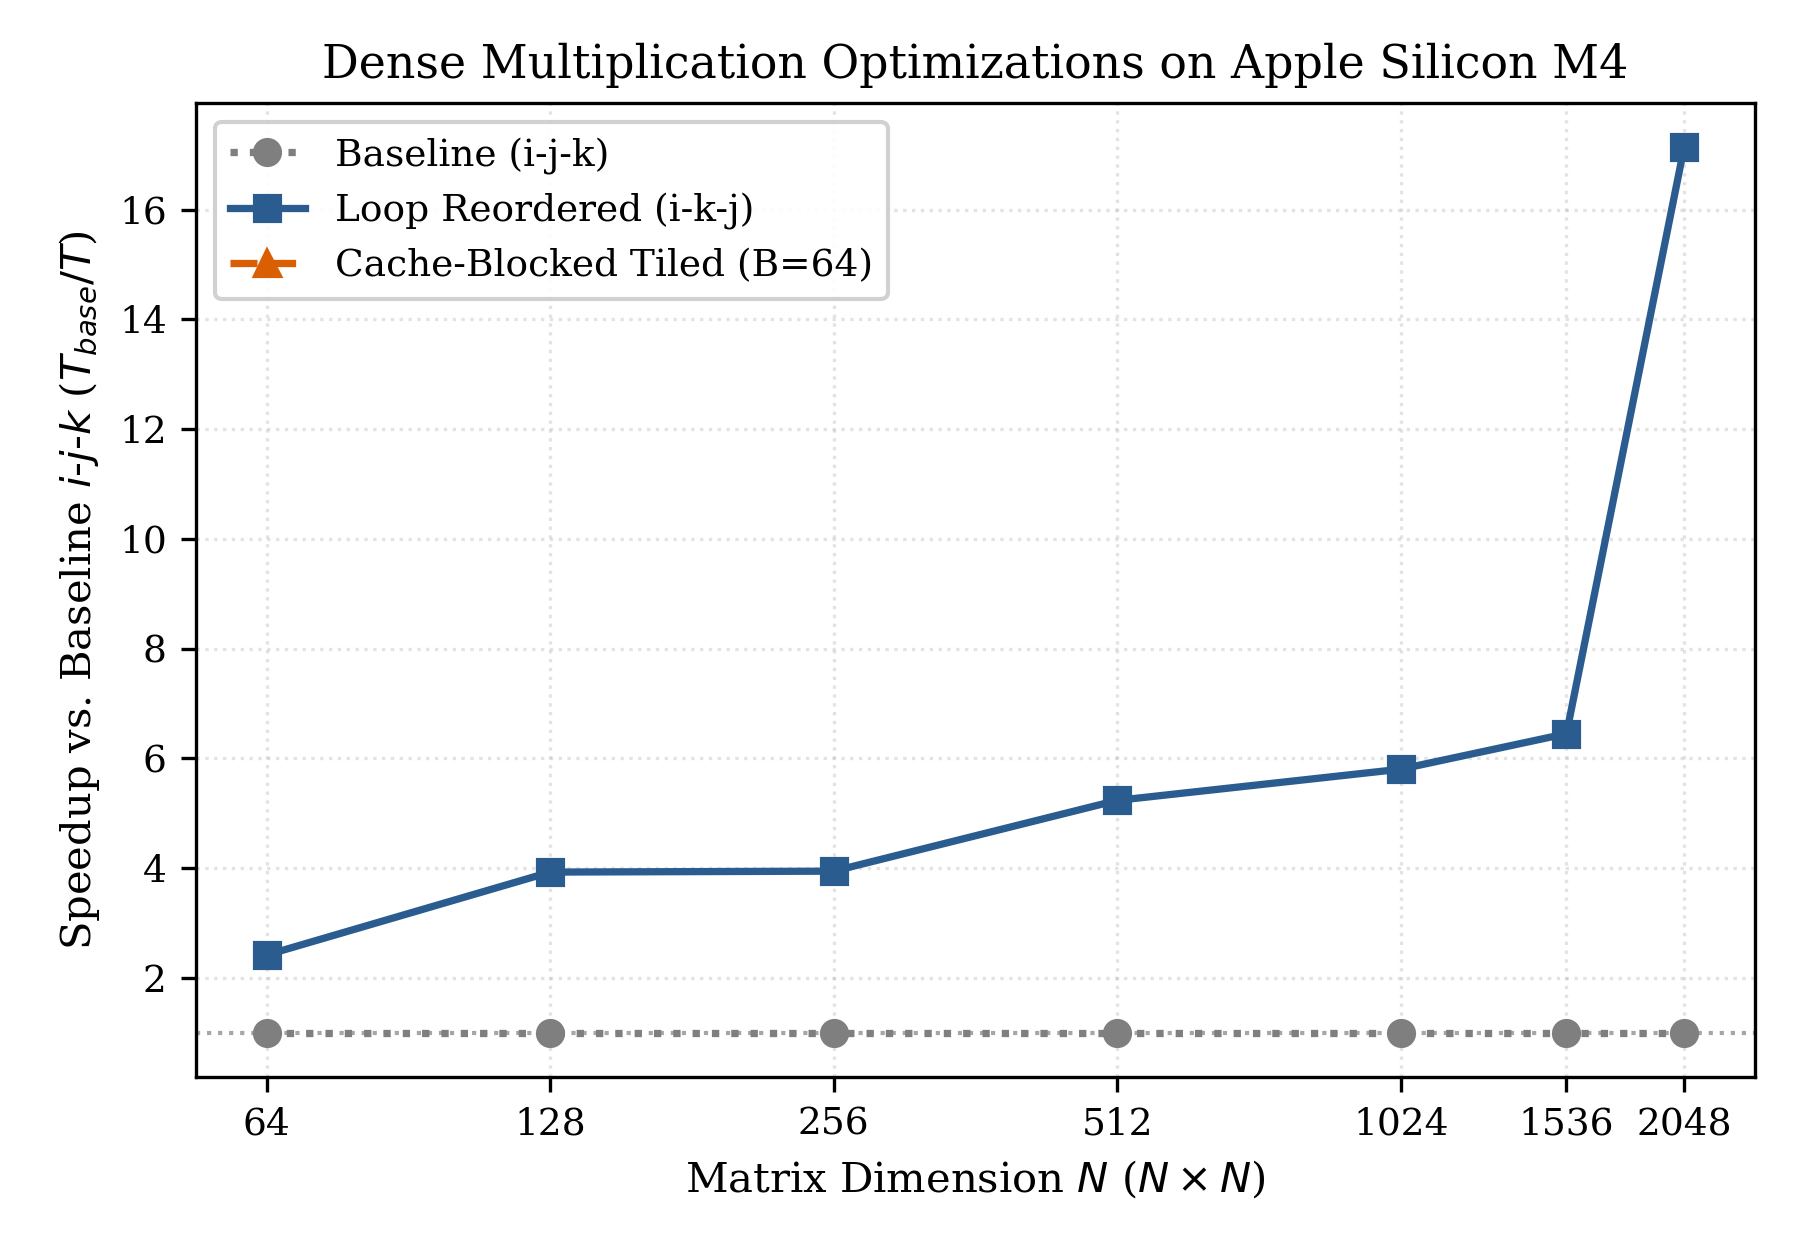
\includegraphics[width=0.92\linewidth]{figures/dense_optimization_speedup.png}
    \caption{Speedup of dense multiplication optimizations over the baseline $i\text{-}j\text{-}k$ implementation.}
    \label{fig:dense_speedup}
\end{figure}

\subsubsection{\texorpdfstring{Baseline $i\text{-}j\text{-}k$ Loop Order}{Baseline i-j-k Loop Order}}
In the standard algorithm, the innermost loop increments $k$:
\begin{equation}
C_{i,j} = \sum_{k=0}^{n-1} A_{i,k} \cdot B_{k,j}
\end{equation}
Reading row $i$ of $A$ moves step by step through memory, but reading column $j$ of $B$ jumps by $n$ elements at every single step. 
For large matrices ($n \ge 512$), this results in each read from $B$ loading a 64-byte line from memory, using only one 8-byte number, and then discarding the remaining 7 numbers before they can be reused. 
So, this results in continuous cache misses.

\subsubsection{\texorpdfstring{Loop Reordering: $i\text{-}k\text{-}j$ Algorithm}{Loop Reordering: i-k-j Algorithm}}
By swapping the two inner loops so that $j$ becomes the innermost loop, the calculation becomes:
\begin{equation}
C_{i,j} \mathrel{+}= A_{i,k} \cdot B_{k,j} \quad \text{for } j = 0, \dots, n-1
\end{equation}
In this arrangement:
\begin{itemize}
    \item The number $A_{i,k}$ does not change during the inner loop and stays in a CPU register.
    \item Both $B_{k,j}$ and $C_{i,j}$ are read and written across index $j$ with a stride of 1, meaning the elements are contiguous in memory.
\end{itemize}
Every cache line loaded for $B$ and $C$ is now used 8 times in a row. 
The CPU hardware prefetcher also detects the sequential reads and pre-loads upcoming cache lines before the code asks for them.

\subsubsection{\texorpdfstring{Cache-Blocked Tiling ($B=64$)}{Cache-Blocked Tiling (B=64)}}
To keep data inside the cache when matrices are large, I also implemented cache-blocked tiling \cite{hennessy2025}. 
The matrices are split into smaller blocks of size $64 \times 64$:
\begin{equation}
B = 64 \implies 64 \times 64 \times 8\,\text{bytes} = 32\,\text{KB}
\end{equation}
Three blocks ($A_{\text{tile}}$, $B_{\text{tile}}$, $C_{\text{tile}}$) take $96\,\text{KB}$, which fits inside the 128 KB L1 data cache of each M4 core. 
Inside each tile, an $i\text{-}k\text{-}j$ loop order is used to keep the stride 1 access.

\subsection{Dense Experimental Results}
Table~\ref{tab:dense_results} and Figure~\ref{fig:dense_speedup} show the measured runtimes as medians of 5 runs and the speedup factors.

\begin{table}[t]
\centering
\caption{Dense Matrix Multiplication Runtime (compiled with Clang \texttt{-O3 -fno-vectorize})}
\label{tab:dense_results}
\setlength{\tabcolsep}{3.2pt}
\footnotesize
\begin{tabular}{r ccc c}
\toprule
$n$ & Baseline $i\text{-}j\text{-}k$ & Reordered $i\text{-}k\text{-}j$ & Tiled ($B=64$) & Speedup \\
    & Median [s] & Median [s] & Median [s] & ($i\text{-}k\text{-}j$ vs Base) \\
\midrule
64   & $0.000179$ & $0.000074$ & $0.000232$ & $2.42\times$ \\
128  & $0.002228$ & $0.000567$ & $0.002024$ & $3.93\times$ \\
256  & $0.020551$ & $0.005208$ & $0.015152$ & $3.95\times$ \\
512  & $0.208964$ & $0.039908$ & $0.086622$ & $5.24\times$ \\
1024 & $1.757119$ & $0.302719$ & $0.697463$ & $5.80\times$ \\
1536 & $6.548821$ & $1.015170$ & $2.317265$ & $6.45\times$ \\
2048 & $40.993368$ & $2.392013$ & $5.266039$ & $\mathbf{17.14\times}$ \\
\bottomrule
\end{tabular}
\end{table}

\subsection{Findings and Discussion}
The measurements show performance differences across the three dense methods:
\begin{itemize}
    \item At $n=512$, $i\text{-}k\text{-}j$ is $5.24\times$ faster than the baseline.
    \item At $n=2048$, three dense matrices take $3 \times 2048^2 \times 8\,\text{bytes} = 96\,\text{MB}$, which is larger than the 16 MB shared L2 cache. The baseline $i\text{-}j\text{-}k$ runtime jumps to $40.99\,\text{s}$ because it constantly has to wait on main memory.
    \item The reordered $i\text{-}k\text{-}j$ implementation finishes in $2.39\,\text{s}$. This results in a speedup of $17.14\times$.
\end{itemize}

An interesting finding is that simple loop reordering ($i\text{-}k\text{-}j$) ran faster than $64\times 64$ tiling ($2.39\,\text{s}$ vs. $5.27\,\text{s}$ at $n=2048$). 
The hardware prefetcher was very effective at streaming long rows of 2048 elements ($16\,\text{KB}$ at a time), so the sequential row streaming achieved better performance than tiled blocking.

\section{Part B: Sparse Matrix Multiplication}

\subsection{Compressed Sparse Row (CSR) Format}
When matrices contain many zeros, storing all numbers in a 2D grid wastes memory and multiplying zeros ($0 \times x = 0$) wastes CPU time.

\begin{figure}[t]
    \centering
    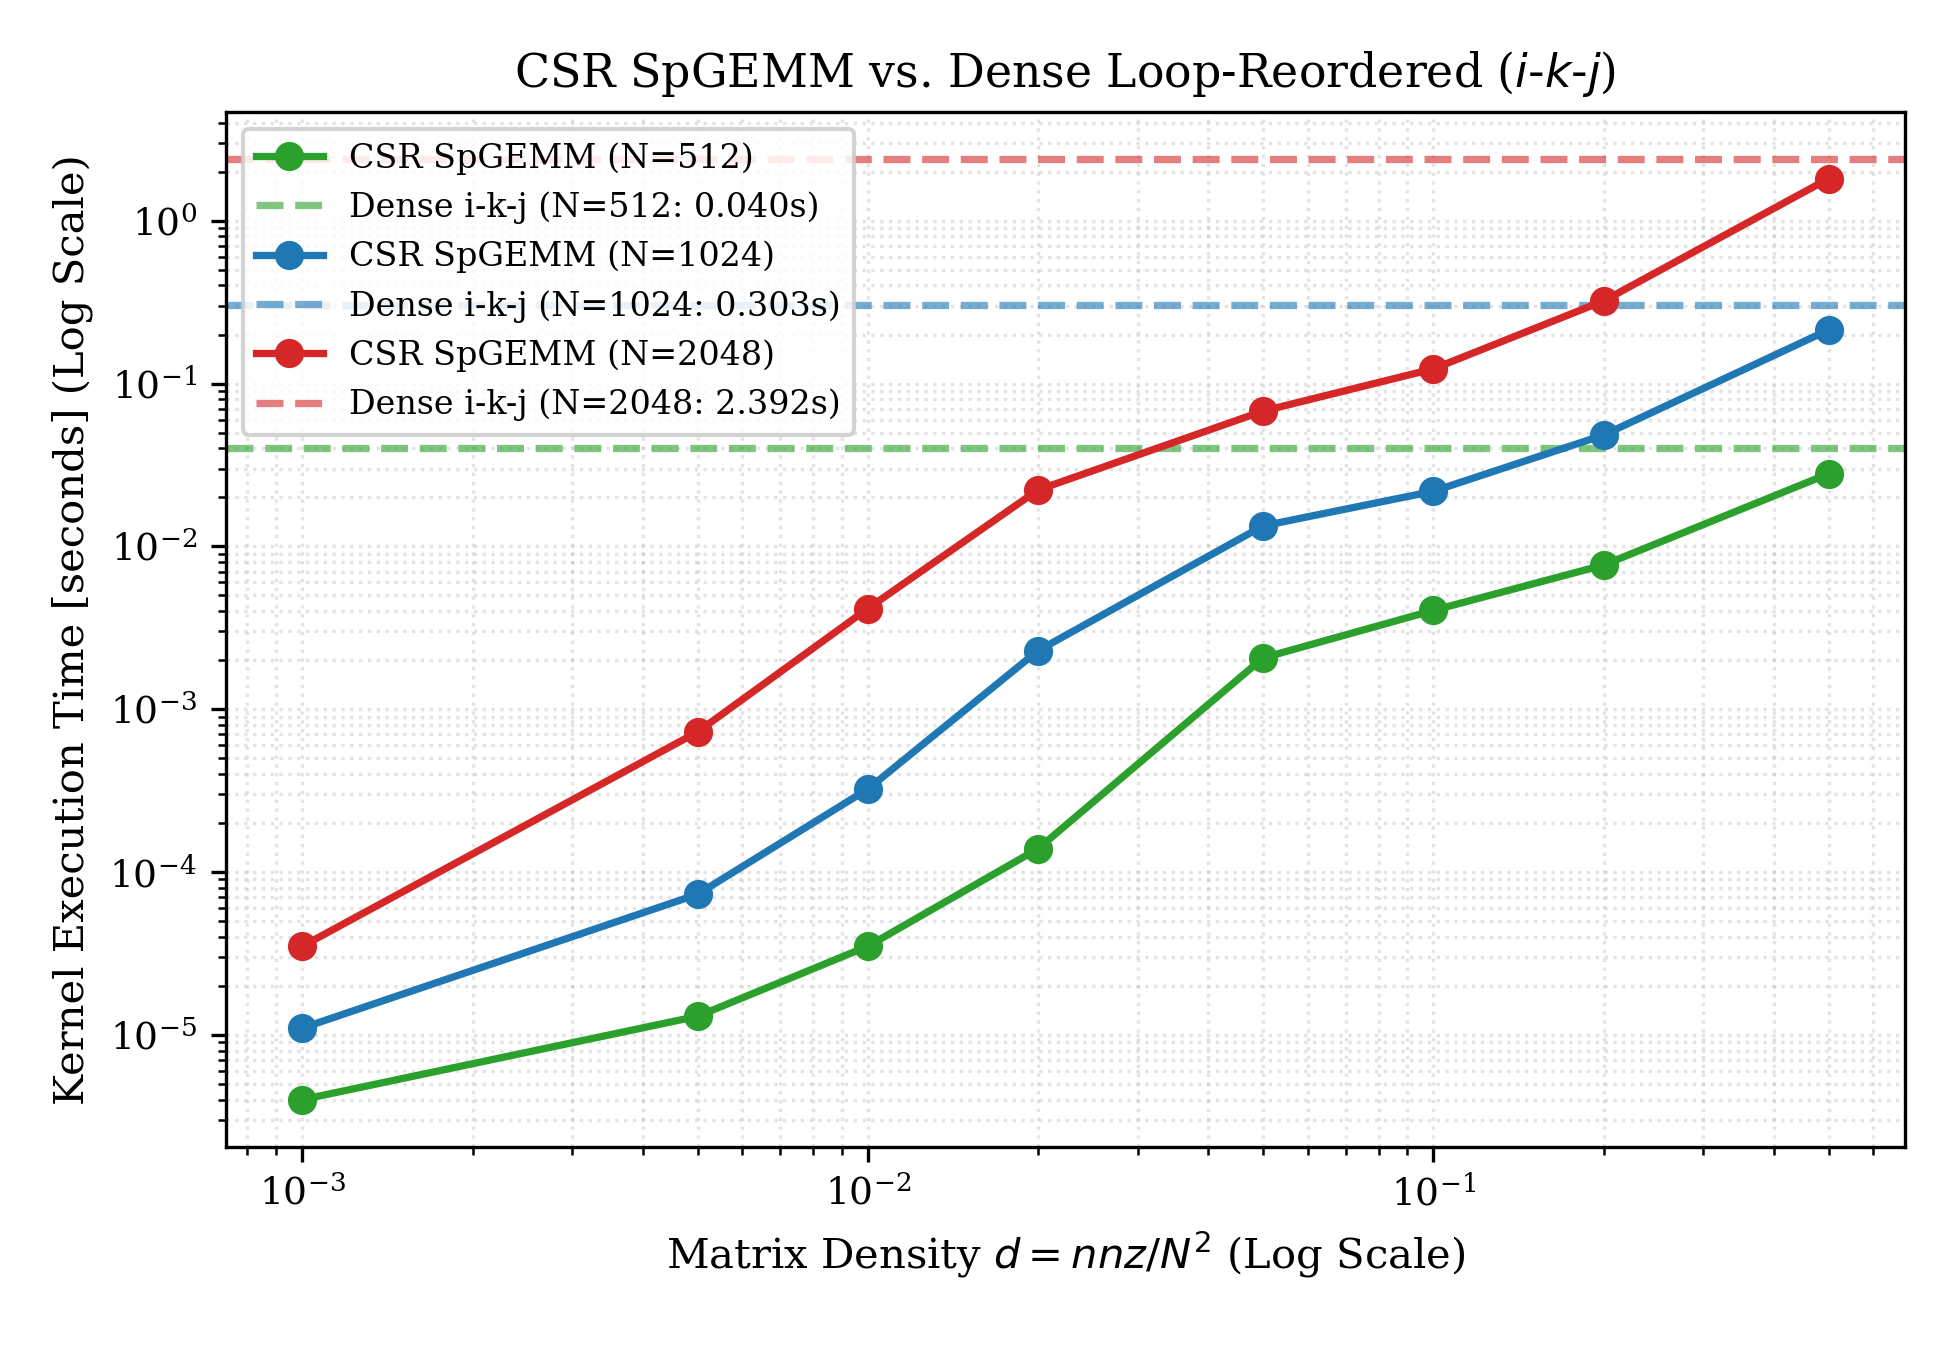
\includegraphics[width=0.92\linewidth]{figures/runtime_vs_sparsity.png}
    \caption{Runtime of CSR SpGEMM across matrix densities compared to dense baselines ($n \in \{512, 1024, 2048\}$) on a log-log scale.}
    \label{fig:runtime_sparsity}
\end{figure}

The Compressed Sparse Row (CSR) format \cite{saad2003, davis2006} stores only the non-zero elements using three 1D arrays:
\begin{enumerate}
    \item \texttt{values} ($nnz$ doubles, 8 bytes each): The non-zero values stored row by row.
    \item \texttt{col\_indices} ($nnz$ integers, 4 bytes each): The column index for each non-zero value.
    \item \texttt{row\_ptr} ($n+1$ integers, 4 bytes each): Pointers showing where each row starts, with \texttt{row\_ptr[n]} $= nnz$.
\end{enumerate}

\subsection{Memory Comparison and Break-Even Point}
The total memory used by an $n \times n$ matrix in CSR format is:
\begin{equation}
M_{\text{CSR}} = 8 \cdot nnz + 4 \cdot nnz + 4(n + 1) = 12 \cdot nnz + 4(n + 1)\,\text{bytes}
\end{equation}
A standard dense 2D array always takes:
\begin{equation}
M_{\text{dense}} = 8 \cdot n^2\,\text{bytes}
\end{equation}

Using density $d = nnz / n^2$, the memory ratio is:
\begin{equation}
\frac{M_{\text{CSR}}}{M_{\text{dense}}} = \frac{12 d n^2 + 4(n+1)}{8 n^2} \approx 1.5 d
\end{equation}
Setting this ratio to $1.0$ gives the theoretical memory break-even density:
\begin{equation}
1.5 d^* = 1.0 \implies d^* = \frac{2}{3} \approx 66.67\% \quad (\text{sparsity } s^* \approx 33.33\%)
\end{equation}
When density is below $66.7\%$, CSR uses less memory than a dense array. 
When density is above $66.7\%$, the extra 4-byte column indices make CSR use more memory than dense storage.

\subsection{Gustavson's SpGEMM Algorithm}
Multiplying two sparse matrices $C = A \cdot B$ is challenging because we do not know in advance where the non-zero entries of $C$ will land. 
I used Gustavson's row-based SpGEMM algorithm \cite{gustavson1978}, which computes $C$ one row at a time:
\begin{enumerate}
    \item For row $i$ of $A$, iterate only over the non-zero entries $A_{i,k}$.
    \item For each $A_{i,k}$, loop through row $k$ of $B$ and multiply $A_{i,k} \cdot B_{k,j}$.
    \item Add the results directly into a temporary array \texttt{accum[j]}.
    \item A helper array \texttt{marker[j]} tracks which columns have already been touched in row $i$ and an \texttt{active\_cols} list keeps track of occupied indices.
    \item Once row $i$ is finished, the non-zeros from \texttt{accum} are written into matrix $C$, and \texttt{accum} is reset for the next row.
\end{enumerate}
This method avoids searching through columns and runs in $O(nnz(A) + \text{flops})$ time.

\subsection{Experimental Results}

\begin{figure}[t]
    \centering
    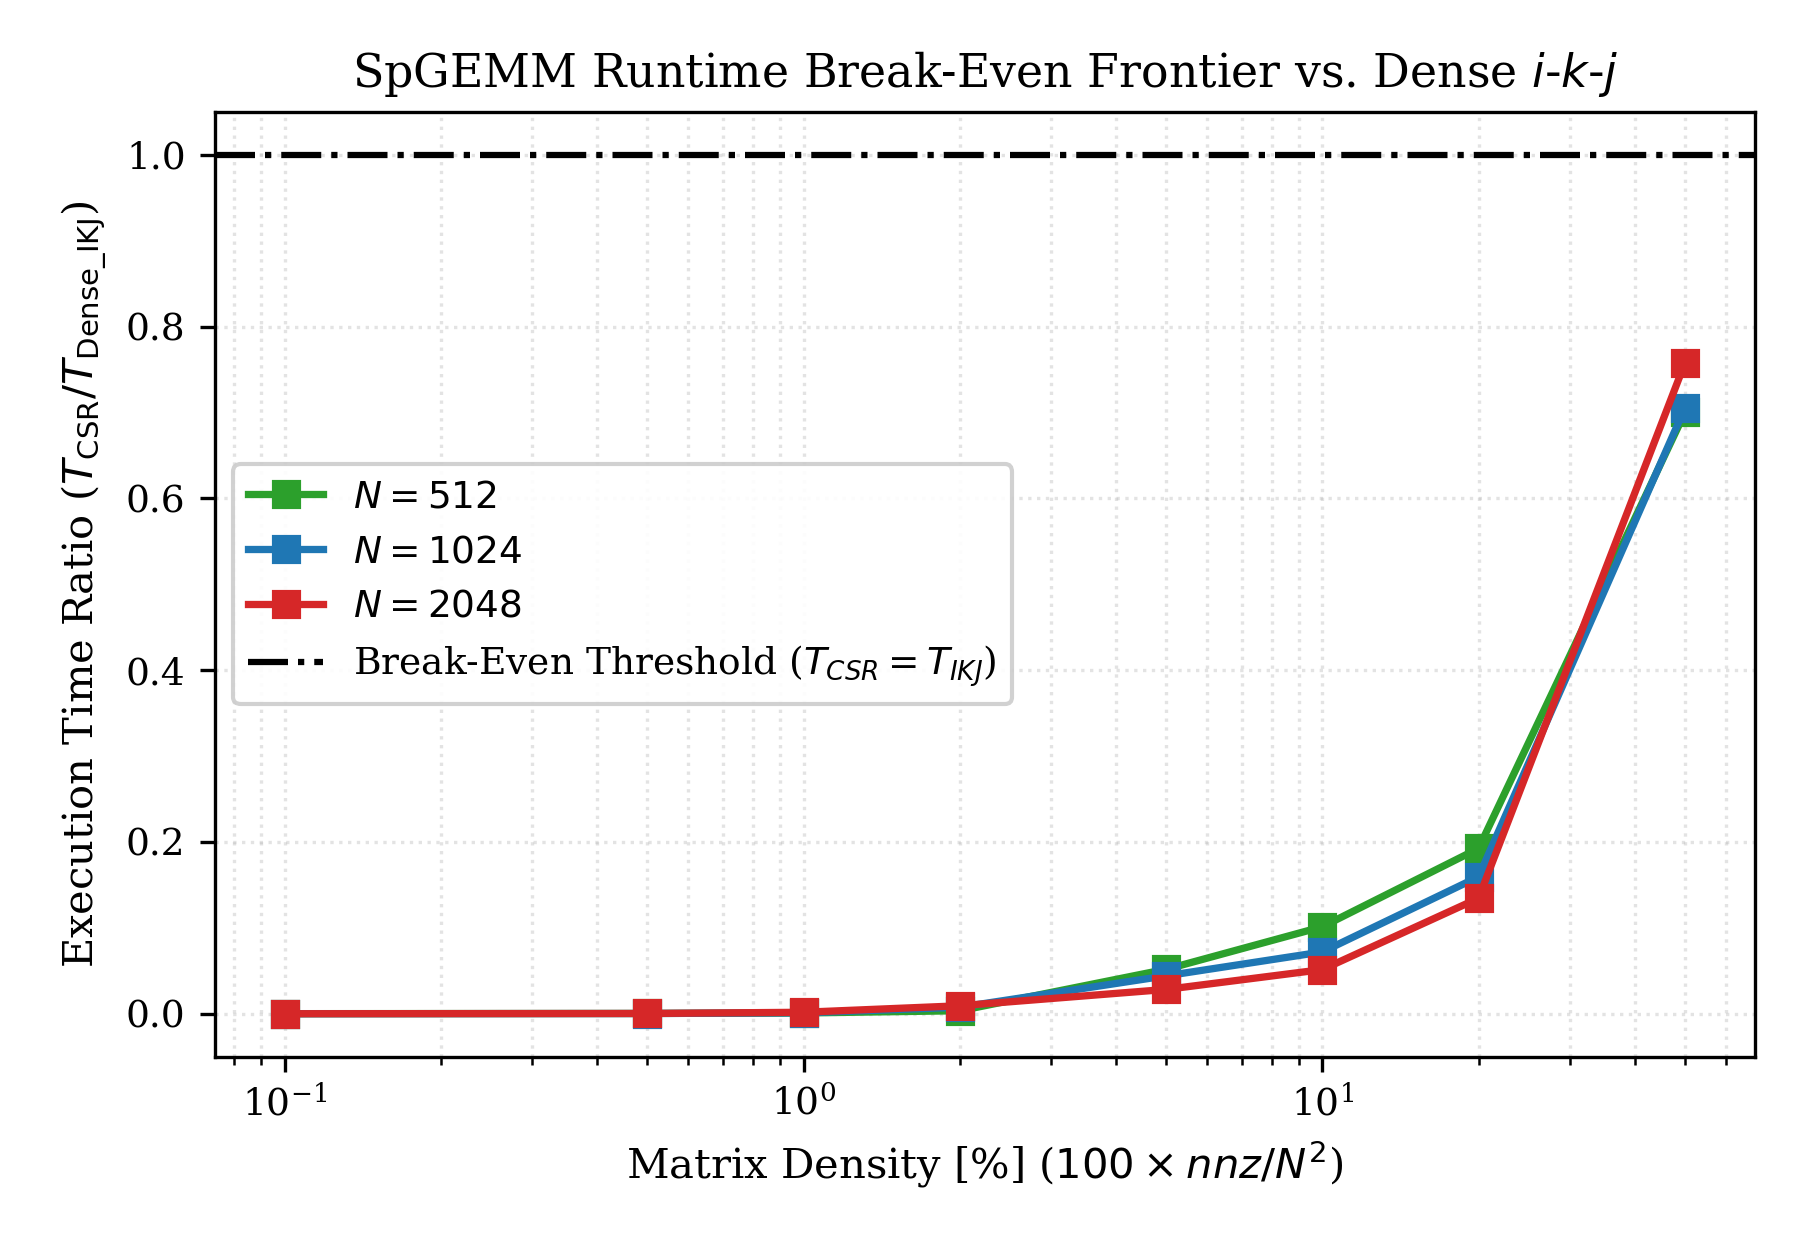
\includegraphics[width=0.92\linewidth]{figures/sparse_breakeven_frontier.png}
    \caption{Runtime ratio ($T_{\text{CSR}} / T_{\text{Dense\_IKJ}}$) across densities. Values below 1.0 mean CSR SpGEMM runs faster than dense $i\text{-}k\text{-}j$.}
    \label{fig:breakeven}
\end{figure}

\begin{figure}[t]
    \centering
    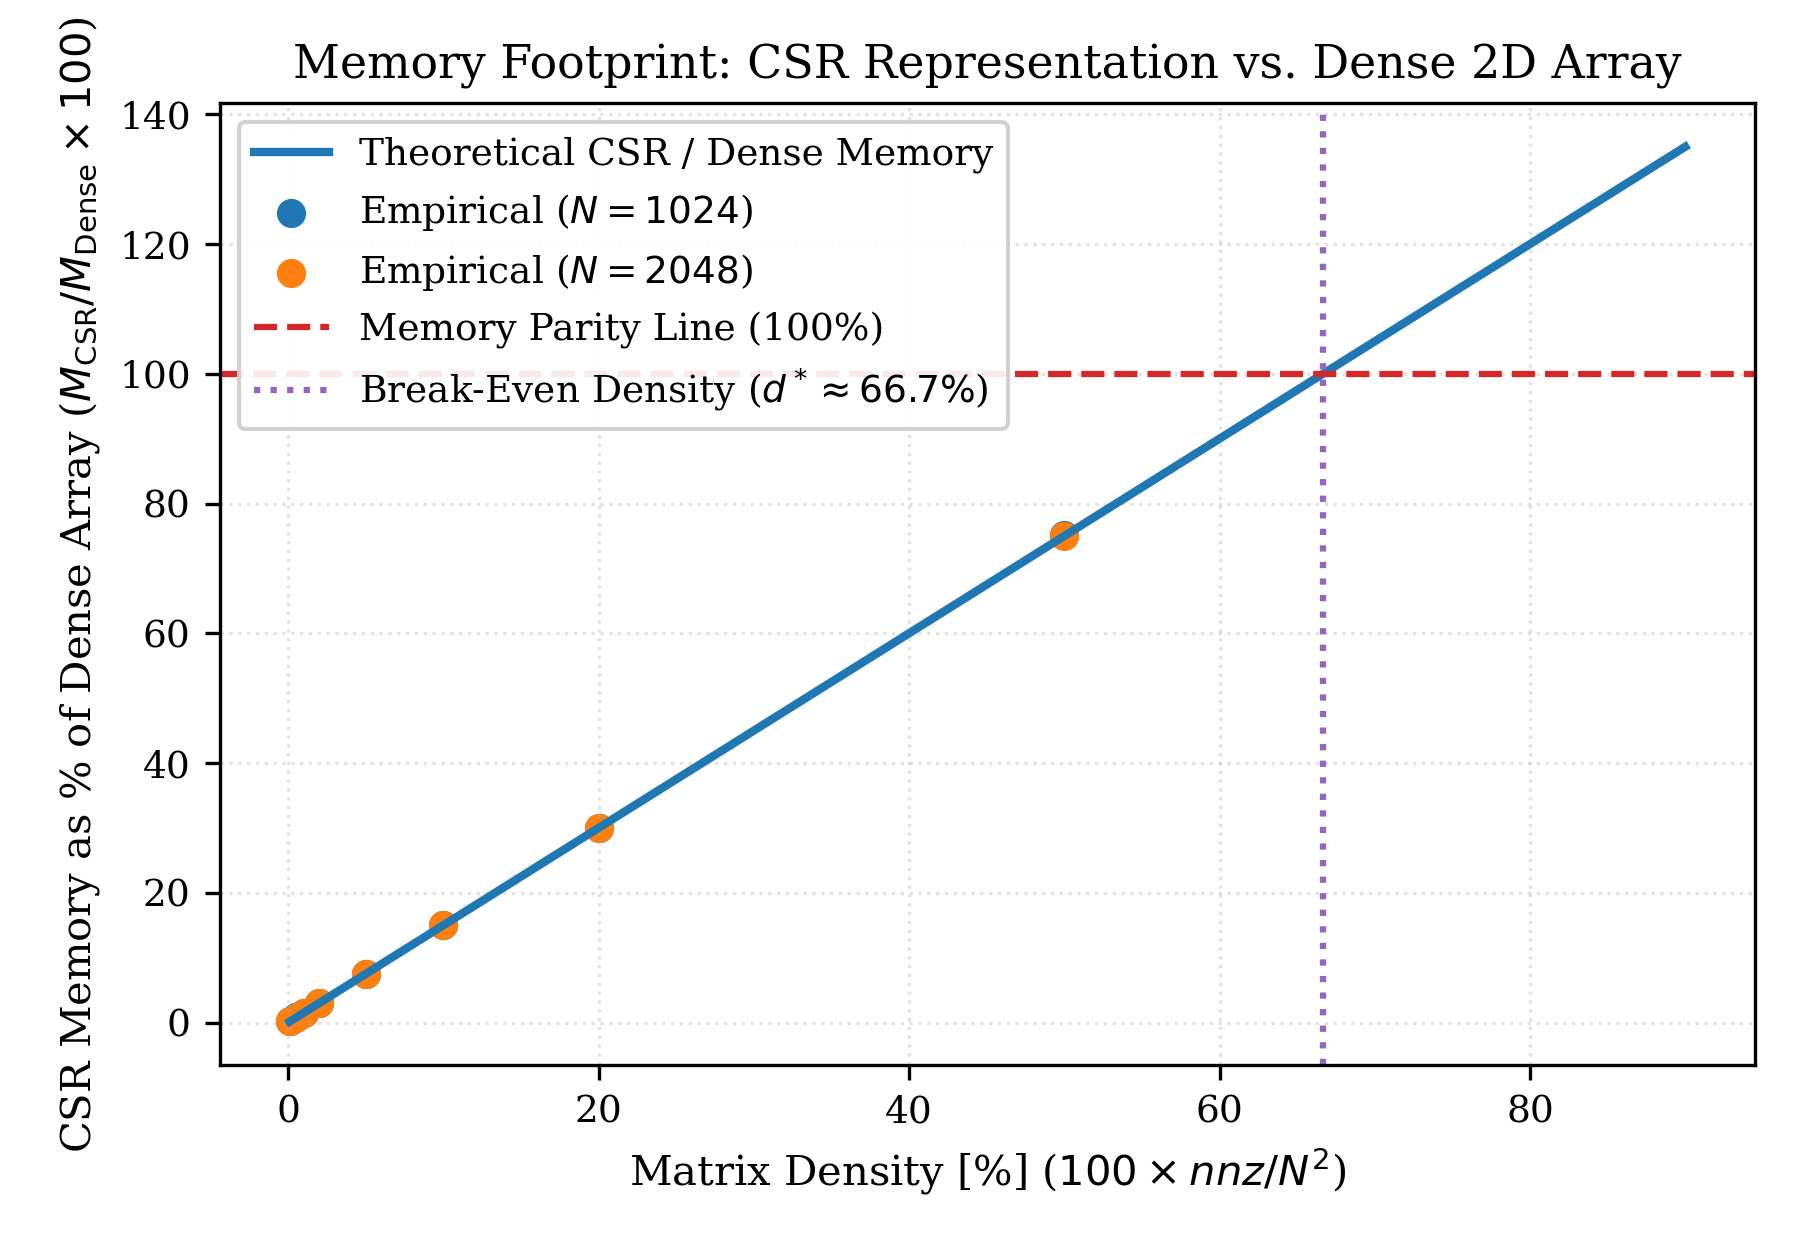
\includegraphics[width=0.92\linewidth]{figures/memory_dense_vs_sparse.png}
    \caption{Memory footprint of CSR vs. dense array across densities. This confirms the theoretical break-even density at $d^* \approx 66.7\%$.}
    \label{fig:memory_curve}
\end{figure}

Table~\ref{tab:sparse_results} shows the performance of CSR SpGEMM at $n=2048$ for densities from $0.1\%$ ($d=0.001$) to $50\%$ ($d=0.50$). 
Figures~\ref{fig:runtime_sparsity}, \ref{fig:breakeven}, and \ref{fig:memory_curve} show the runtime comparisons, break-even curves and memory usage.

\begin{table}[t]
\centering
\caption{CSR SpGEMM Runtime and Comparison with Dense at $n=2048$}
\label{tab:sparse_results}
\setlength{\tabcolsep}{2.8pt}
\footnotesize
\begin{tabular}{r ccc cc}
\toprule
Density & Sparsity & SpGEMM & CSR Mem & Mem & Speedup vs \\
$d$ & $1-d$ & Median [s] & [KB] & Savings & Dense $i\text{-}k\text{-}j$ \\
\midrule
$0.001$ & $99.9\%$ & $0.000035$ & $116$ & $99.82\%$ & $\mathbf{68{,}343\times}$ \\
$0.005$ & $99.5\%$ & $0.000725$ & $508$ & $99.22\%$ & $\mathbf{3{,}299\times}$ \\
$0.010$ & $99.0\%$ & $0.004149$ & $1{,}000$ & $98.47\%$ & $\mathbf{576\times}$ \\
$0.020$ & $98.0\%$ & $0.022211$ & $1{,}979$ & $96.98\%$ & $\mathbf{107\times}$ \\
$0.050$ & $95.0\%$ & $0.067753$ & $4{,}932$ & $92.47\%$ & $\mathbf{35.3\times}$ \\
$0.100$ & $90.0\%$ & $0.123052$ & $9{,}849$ & $84.97\%$ & $\mathbf{19.4\times}$ \\
$0.200$ & $80.0\%$ & $0.321737$ & $19{,}671$ & $69.98\%$ & $\mathbf{7.43\times}$ \\
$0.500$ & $50.0\%$ & $1.813037$ & $49{,}174$ & $24.97\%$ & $\mathbf{1.32\times}$ \\
\bottomrule
\end{tabular}
\end{table}

\subsection{Findings}
The benchmark results show three main insights:

\subsubsection{Large Speedups at High Sparsity}
When matrices have few non-zeros ($d \le 0.01$, or $99\%$ sparse), SpGEMM runs in a few milliseconds ($4.15\,\text{ms}$ at $d=0.01$, $n=2048$). 
This is $576\times$ faster than the optimized dense $i\text{-}k\text{-}j$ code and $9{,}880\times$ faster than the baseline $i\text{-}j\text{-}k$ code. 
At $d=0.001$, the speedup reaches $68{,}343\times$.

\subsubsection{Sparsity of the output matrix}
When multiplying two sparse matrices, the output matrix $C$ usually ends up less sparse than the input matrices. 
At $n=2048$ with $d=0.01$, matrices $A$ and $B$ have around $42{,}000$ non-zeros each ($1\%$ density). 
However, their product $C$ contains $779{,}173$ non-zeros, an $18.6\times$ increase in non-zeros.

By $d=0.10$ ($10\%$ non-zeros in $A$ and $B$), matrix $C$ contains $4{,}194,304$ non-zeros, meaning it is $100\%$ full. 
Even though the output is fully dense, Gustavson's SpGEMM finishes in $0.123\,\text{s}$, which is still $19.4\times$ faster than the dense $i\text{-}k\text{-}j$ kernel ($2.39\,\text{s}$). 
This happens because the algorithm only loops over the $10\%$ non-zero entries in $A$ and $B$.

\subsubsection{Runtime Break-Even Point}
As density rises to $d=0.50$, SpGEMM runtime increases to $1.81\,\text{s}$, getting closer to the $2.39\,\text{s}$ runtime of dense $i\text{-}k\text{-}j$ (ratio $T_{\text{CSR}} / T_{\text{Dense}} \approx 0.76$). 
Looking at the curve in Figure~\ref{fig:breakeven}, the runtime break-even point occurs around $d \approx 55\% - 65\%$. 
Above this density, the extra work of aspects such as checking indices, following pointers and resizing buffers takes more time than what is saved by skipping zeros.

\section{Limitations}
\begin{itemize}
    \item The test matrices used uniformly distributed random non-zero positions. 
    Real-world sparse matrices (such as in social network graphs) often have clustered structures, which can change cache performance.
    \item All benchmarks were run focusing on memory access patterns, so only on one CPU core and without SIMD vectorization, therefore not a real world scenario.
\end{itemize}

\section{Conclusions}
This evaluation shows the following takeaways for matrix multiplication:
\begin{enumerate}
    \item \textbf{Always use $i\text{-}k\text{-}j$ for dense multiplication:} Swapping two loop lines to create continuous memory reads (with stride 1) gave a $17.14\times$ speedup at $n=2048$, without requiring extra memory.
    \item \textbf{Sequential streaming can be faster than tiling:} On processors with large L1 caches and fast hardware prefetchers, simple sequential row reads can run faster than cache-blocked tiling because they avoid extra loop overhead and keep memory streaming smoothly.
    \item \textbf{When to use CSR SpGEMM:} Sparse CSR multiplication provides large speedups (from $35\times$ up to $68{,}000\times$) when density is low ($d \le 0.05$). 
    The memory break-even point is $66.7\%$ density and the runtime break-even point is around $55\% - 65\%$. 
    Therefore, if a matrix has more than $60\%$ non-zero values, dense $i\text{-}k\text{-}j$ is usually the better option.
\end{enumerate}

\bibliographystyle{IEEEtran}
\begin{thebibliography}{10}
\bibitem{golub2013}
G.~H. Golub and C.~F. Van~Loan, \emph{Matrix Computations}, 3rd~ed.\hskip 1em plus 0.5em minus 0.4em\relax Johns Hopkins University Press, 2013.

\bibitem{ulpgc2026}
ULPGC, ``Individual Assignments: Matrix Multiplication,'' \emph{Big Data Course Specification}, Universidad de Las Palmas de Gran Canaria, 2026--2027.

\bibitem{bigdataweb}
ULPGC, ``Big Data Course,'' \url{https://mltechdrawer.github.io/BIGDATA/}, [Accessed 30-Oct-2026].

\bibitem{hennessy2025}
J.~L. Hennessy and D.~A. Patterson, \emph{Computer Architecture: A Quantitative Approach}, \hskip 1em plus 0.5em minus 0.4em\relax Morgan Kaufmann, 2025.

\bibitem{saad2003}
Y.~Saad, \emph{Iterative Methods for Sparse Linear Systems}, \hskip 1em plus 0.5em minus 0.4em\relax SIAM, 2003.

\bibitem{davis2006}
T.~A. Davis, \emph{Direct Methods for Sparse Linear Systems}.\hskip 1em plus 0.5em minus 0.4em\relax SIAM, 2006.

\bibitem{gustavson1978}
F.~G. Gustavson, ``Two fast algorithms for sparse matrices: Multiplication and permuted transposition,'' \emph{ACM Transactions on Mathematical Software (TOMS)}, vol.~4, no.~3, pp. 250--269, 1978.

\end{thebibliography}

\end{document}
